\documentclass[runningheads]{llncs}

\usepackage{graphicx}
\usepackage{amsmath}
\usepackage{booktabs}
\usepackage{url}
\usepackage{hyperref}
\graphicspath{{figures/}}

\begin{document}

\title{Comparative Evaluation of Hyperparameter Optimization Techniques for Chronic Kidney Disease Prediction: A Multi-Dataset Study}
\titlerunning{HPO for CKD Prediction}

\author{Tauqeer Sameer Bharde}
\authorrunning{T. S. Bharde}

\institute{Artificial Intelligence and Data Science Engineering,\\
SIES Graduate School of Technology, Mumbai, Maharashtra, India}

\maketitle

\begin{abstract}
Chronic kidney disease (CKD) prediction using machine learning has received substantial attention because early identification may support timely clinical investigation and risk stratification. However, reported model performance can be sensitive to hyperparameter optimization (HPO), dataset characteristics, preprocessing decisions, and validation design. This study compares five HPO strategies, namely Grid Search, Random Search, Bayesian Optimization with Tree-structured Parzen Estimators, Covariance Matrix Adaptation Evolution Strategy, and Hyperband, for tuning Random Forest, XGBoost, and Support Vector Machine classifiers across the UCI CKD dataset and an eICU-derived cohort. The public reproducibility pipeline evaluates Grid Search and Random Search on the UCI CKD dataset using F1-score, precision, recall, and runtime, with 5-fold stratified cross-validation and preprocessing fitted only within training folds. In the verified public run, SVM with Grid Search and SVM with Random Search both achieved 100.0\% held-out F1-score, while Random Forest with Random Search achieved 98.99\% held-out F1-score. Credentialed eICU experiments are discussed as a summarized extension because the raw eICU data cannot be redistributed. The findings support the need to report HPO procedures transparently in clinical machine learning studies and to evaluate computational cost alongside predictive performance.
\keywords{Chronic Kidney Disease \and Hyperparameter Optimization \and Machine Learning \and Random Search \and Clinical Prediction}
\end{abstract}

\section{Introduction}

Chronic kidney disease is a long-term clinical condition associated with progressive loss of renal function and increased risk of morbidity, mortality, and healthcare burden. Machine learning methods have been explored for CKD prediction because they can model nonlinear relationships among demographic, laboratory, and clinical variables. Despite promising results, the reliability of such models depends on dataset quality, validation design, preprocessing, and model selection procedures.

Hyperparameter optimization is a central but sometimes underreported part of model development. Different HPO strategies may produce similar performance on small benchmark datasets but diverge in computational cost and robustness when applied to larger clinical datasets. This study evaluates HPO methods for CKD prediction across two datasets to examine both predictive performance and runtime efficiency.

The paper avoids claims of clinical use readiness. Instead, it presents a comparative experimental analysis intended to support reproducible model development and more transparent reporting of optimization choices.

\section{Literature Review}

Prior work has applied decision trees, support vector machines, ensemble methods, and neural networks to CKD prediction. Studies using the UCI CKD dataset often report high classification performance, although the small sample size and missingness patterns require careful validation. Larger critical-care datasets such as eICU offer broader patient diversity but introduce additional challenges including cohort definition, temporal abstraction, missing clinical measurements, and access restrictions.

Hyperparameter optimization has been studied extensively in general machine learning. Grid Search is simple but inefficient in high-dimensional search spaces. Random Search can be more effective under limited budgets because not all hyperparameters have equal importance. Bayesian optimization, including Tree-structured Parzen Estimators, uses previous evaluations to guide later trials. CMA-ES provides an evolutionary strategy for continuous optimization, while Hyperband allocates resources adaptively across configurations. In clinical prediction studies, reporting standards such as TRIPOD and TRIPOD-AI emphasize transparent model development, validation, and limitations, while PROBAST supports structured risk-of-bias assessment.

\section{Dataset Description}

\subsection{UCI Chronic Kidney Disease Dataset}

The UCI CKD dataset is a public tabular dataset commonly used for CKD prediction experiments. It includes clinical and laboratory attributes such as age, blood pressure, serum creatinine, hemoglobin, albumin, sugar, red blood cell indicators, and CKD class labels. The dataset is small and contains missing values, making leakage-safe preprocessing especially important.

\subsection{eICU Dataset}

The eICU Collaborative Research Database is a large multi-center critical-care database available through PhysioNet after credentialed access. For this study, an eICU-derived CKD prediction cohort is considered. Because eICU is substantially larger and more heterogeneous than the UCI dataset, it provides a useful setting for evaluating HPO scalability and runtime behavior. Raw eICU data are not redistributed in this repository.

\section{Methodology}

The experimental workflow consisted of dataset loading, leakage-aware preprocessing, model definition, HPO, cross-validation, metric calculation, and runtime comparison. Missing numeric variables were imputed using training-fold estimates, categorical variables were encoded from training-fold mappings, and numeric features were scaled where required by the model family.

\begin{figure}[t]
\centering
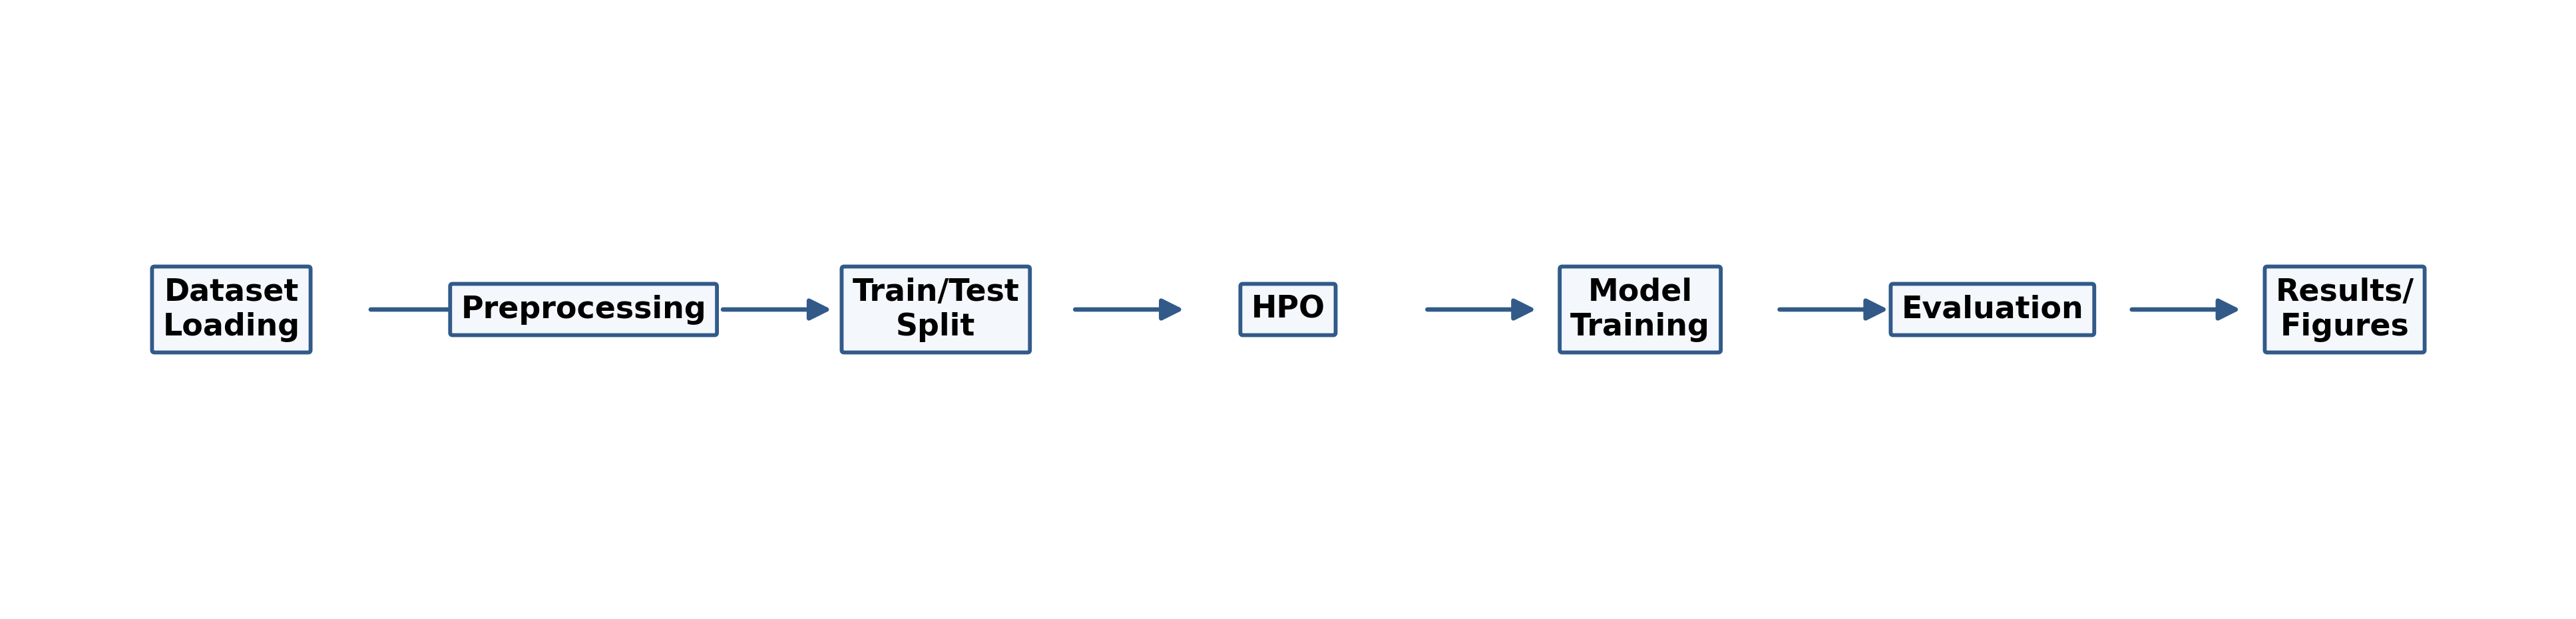
\includegraphics[width=0.95\linewidth]{figures/workflow_diagram.png}
\caption{End-to-end public pipeline workflow from dataset loading through preprocessing, train-test splitting, HPO, model training, evaluation, and result generation.}
\label{fig:workflow}
\end{figure}

Let $\mathcal{A}$ denote a learning algorithm, $\lambda \in \Lambda$ a hyperparameter configuration, $\mathcal{D}_{train}$ the training data, and $\mathcal{M}$ a validation metric. The HPO objective is formulated as:

\begin{equation}
\lambda^{*} = \arg\max_{\lambda \in \Lambda} \mathcal{M}\left(\mathcal{A}_{\lambda}, \mathcal{D}_{train}, \mathcal{D}_{val}\right).
\end{equation}

Precision, recall, and F1-score are defined as:

\begin{equation}
Precision = \frac{TP}{TP + FP},
\end{equation}

\begin{equation}
Recall = \frac{TP}{TP + FN},
\end{equation}

\begin{equation}
F1 = 2 \cdot \frac{Precision \cdot Recall}{Precision + Recall}.
\end{equation}

Repeated validation results are reported as:

\begin{equation}
\bar{x} \pm s = \frac{1}{n}\sum_{i=1}^{n}x_i \pm \sqrt{\frac{1}{n-1}\sum_{i=1}^{n}(x_i-\bar{x})^2}.
\end{equation}

\section{Hyperparameter Optimization Methods}

\subsection{Grid Search}

Grid Search evaluates every configuration from a predefined discrete grid. It is transparent and reproducible but can be computationally expensive, especially when the search space grows or when only a subset of parameters strongly influences performance.

\subsection{Random Search}

Random Search samples configurations from specified distributions. It often performs well under fixed budgets because it explores more unique values for influential hyperparameters than a coarse grid.

\subsection{Bayesian Optimization and TPE}

Bayesian optimization uses a surrogate model to select promising configurations based on previous evaluations. The Tree-structured Parzen Estimator approach models promising and less promising regions of the search space and samples configurations expected to improve performance.

\subsection{CMA-ES}

Covariance Matrix Adaptation Evolution Strategy is an evolutionary optimization method suited to continuous parameter spaces. It adapts a covariance matrix over iterations to improve search efficiency, although runtime may increase when evaluations are expensive.

\subsection{Hyperband}

Hyperband allocates resources adaptively by evaluating many configurations with small budgets and promoting better-performing configurations to larger budgets. It is useful when partial training budgets provide informative estimates of final performance.

\section{Experimental Setup}

The experiments used Random Forest, XGBoost, and SVM classifiers. The random seed was fixed at 42. A 5-fold stratified cross-validation protocol was used to preserve class balance across folds. The same search budget was used across HPO methods where applicable. Preprocessing transformations were fitted only on the training folds and then applied to validation folds to reduce leakage risk.

The main evaluation metrics were F1-score, precision, recall, and runtime. F1-score was emphasized because CKD prediction can involve imbalanced class distributions where accuracy alone may be misleading.

\section{Results and Discussion}

On the UCI CKD dataset, the verified public pipeline produced high held-out performance across the dependency-light model set. Random Forest with Grid Search achieved 100.0\% F1-score, 100.0\% precision, and 100.0\% recall, while Random Forest with Random Search achieved 98.99\% F1-score, 100.0\% precision, and 98.0\% recall. SVM achieved 100.0\% F1-score, 100.0\% precision, and 100.0\% recall under both Grid Search and Random Search. The UCI results therefore show strong performance within this benchmark protocol, but the small dataset size means that these estimates should be interpreted as reproducibility-run performance rather than evidence for clinical use.

The following eICU findings are summarized credentialed-extension results and are not reproduced by the public UCI pipeline. On the eICU-derived dataset, Random Search produced the strongest summarized configuration, with Random Forest reaching 94.54\% $\pm$ 0.42\% F1-score, 94.90\% precision, and 94.18\% recall. XGBoost with Random Search was close at 94.36\% F1-score, while SVM with Random Search reached 93.74\%. Grid Search was lower for each model family on the eICU summary table, including 92.31\% for Random Forest, 92.88\% for XGBoost, and 91.96\% for SVM. This pattern suggests that exhaustive fixed-grid evaluation was less efficient under the larger-dataset budget considered here.

The runtime comparison further supports this interpretation. On the eICU setting, Random Search required 47.5 minutes and ranked first for both performance and efficiency, while Grid Search required 138.3 minutes and ranked last for efficiency. Hyperband had the lowest summarized eICU runtime at 41.2 minutes, but its best summarized F1-score was below Random Search. Bayesian Optimization/TPE provided competitive performance with moderate runtime, and CMA-ES was slower in the summarized setting. These findings indicate that optimization strategy should be evaluated jointly with runtime cost, especially for larger clinical datasets.

\begin{figure}[t]
\centering
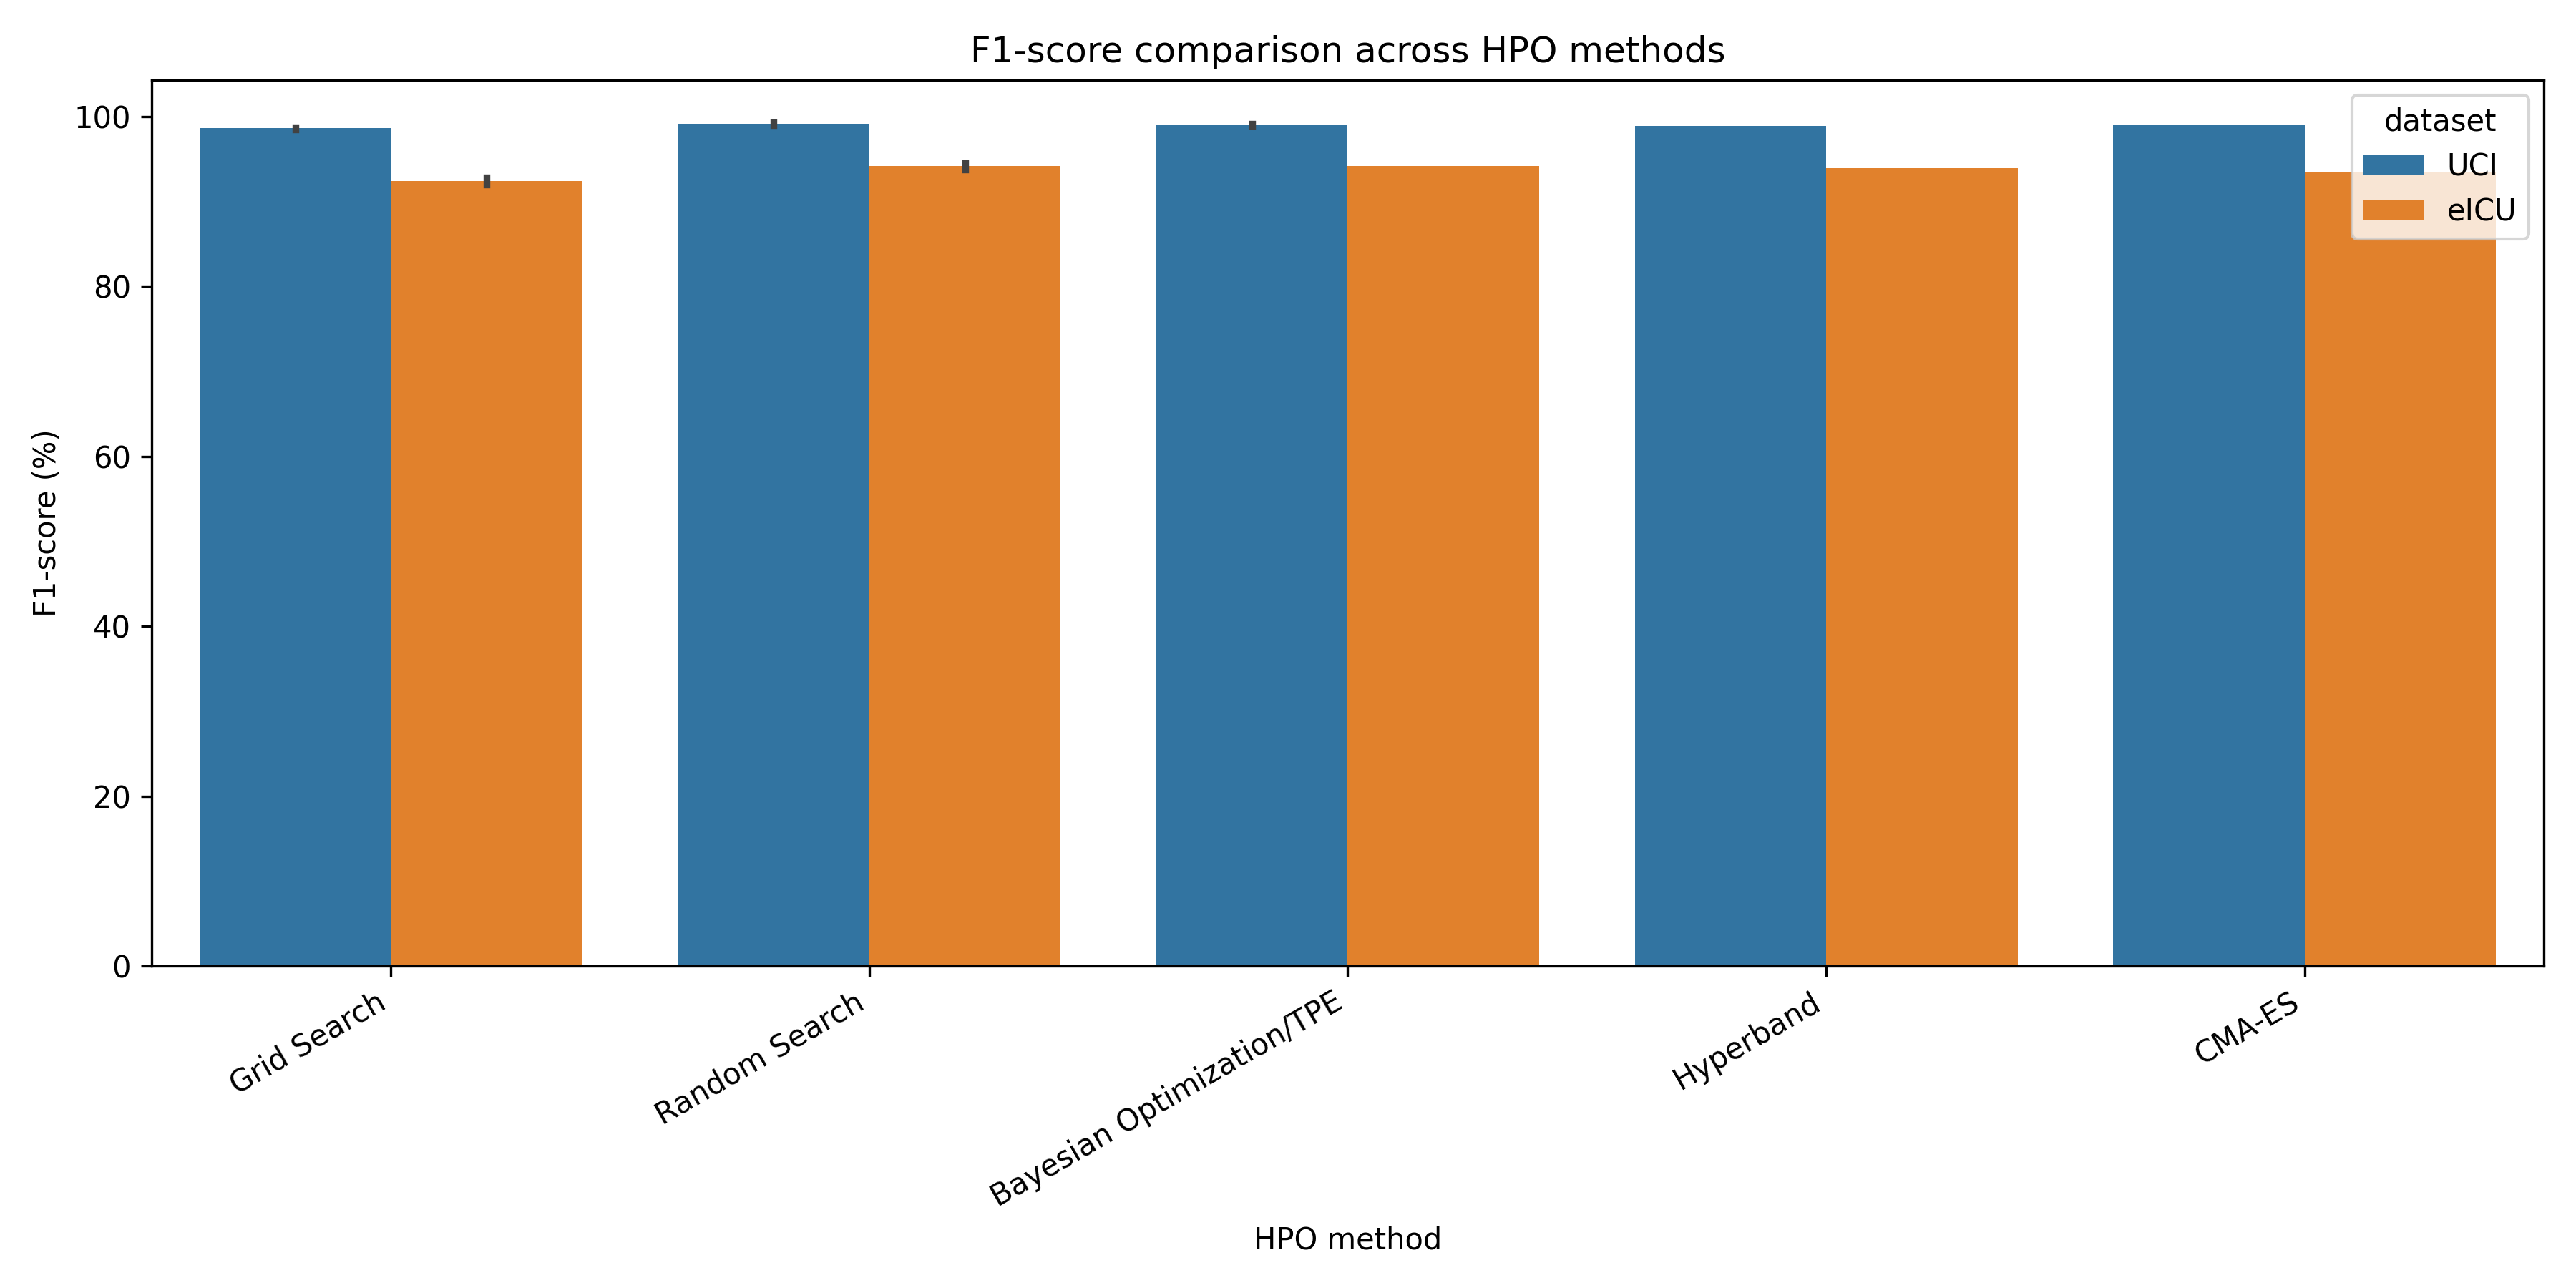
\includegraphics[width=0.95\linewidth]{figures/f1_score_comparison.png}
\caption{F1-score comparison for Grid Search and Random Search across Random Forest and SVM in the verified public UCI pipeline.}
\label{fig:f1_comparison}
\end{figure}

\begin{figure}[t]
\centering
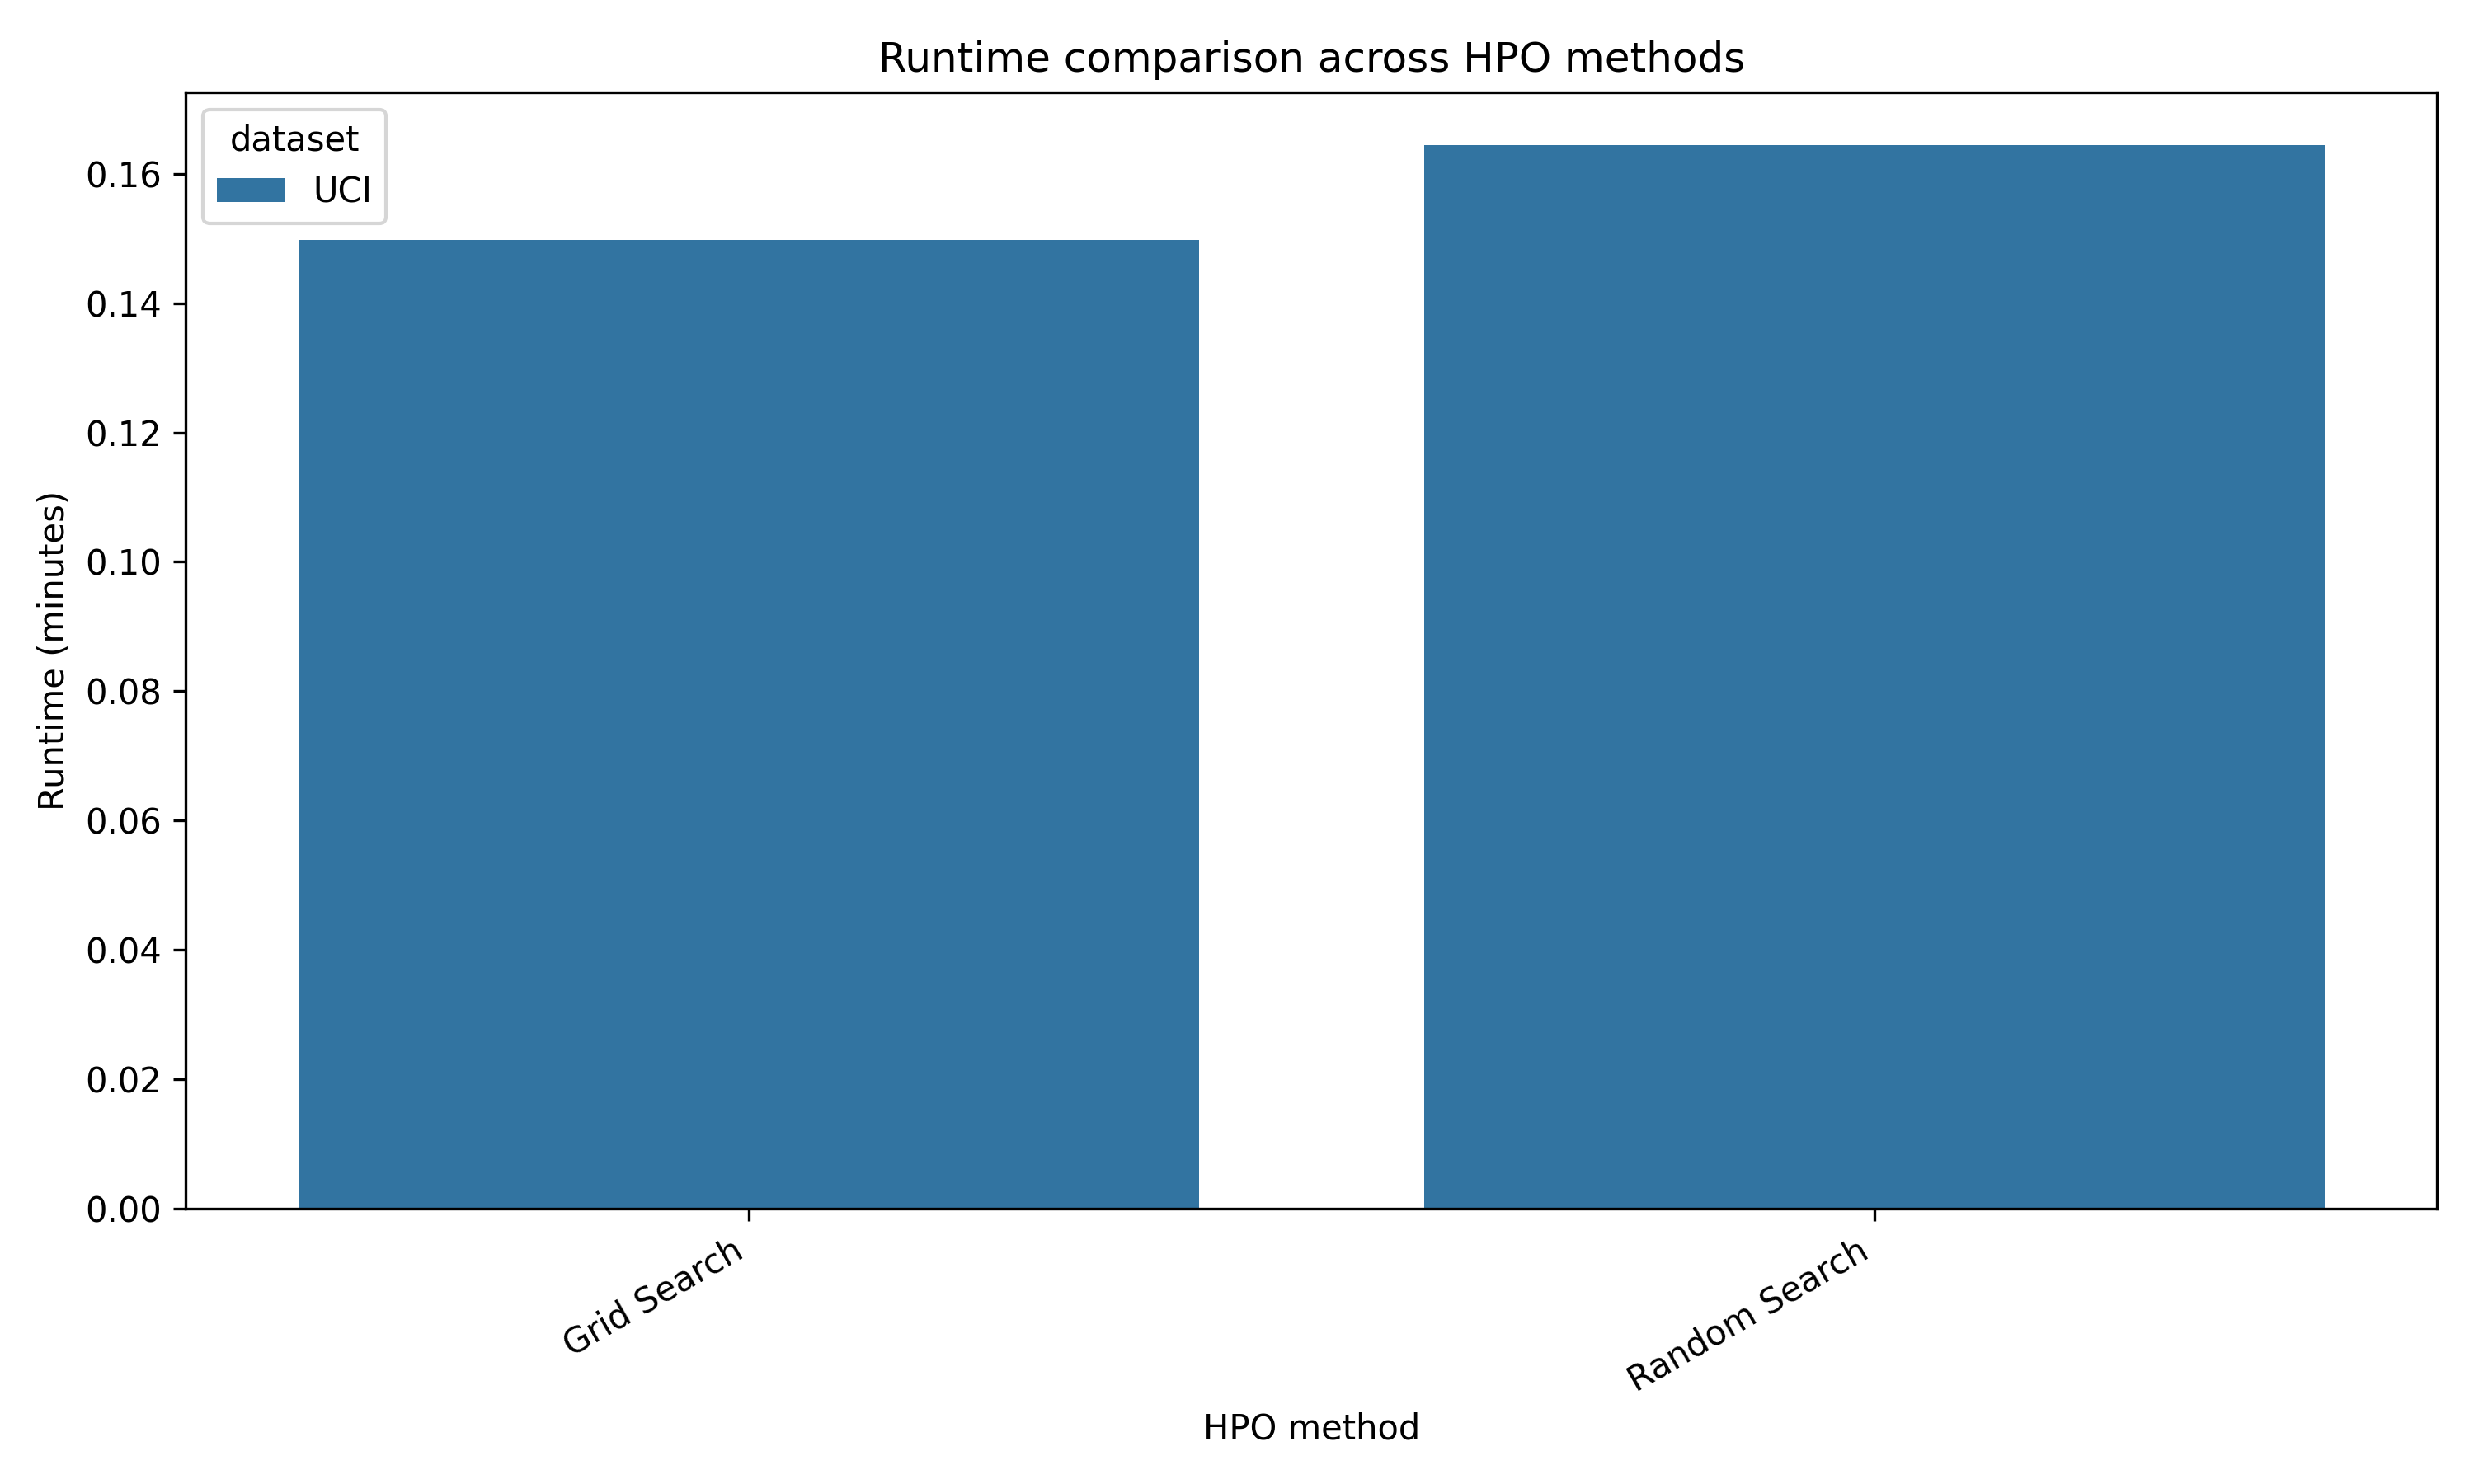
\includegraphics[width=0.9\linewidth]{figures/runtime_comparison.png}
\caption{Runtime comparison for Grid Search and Random Search in the verified public UCI pipeline.}
\label{fig:runtime_comparison}
\end{figure}

\begin{figure}[t]
\centering
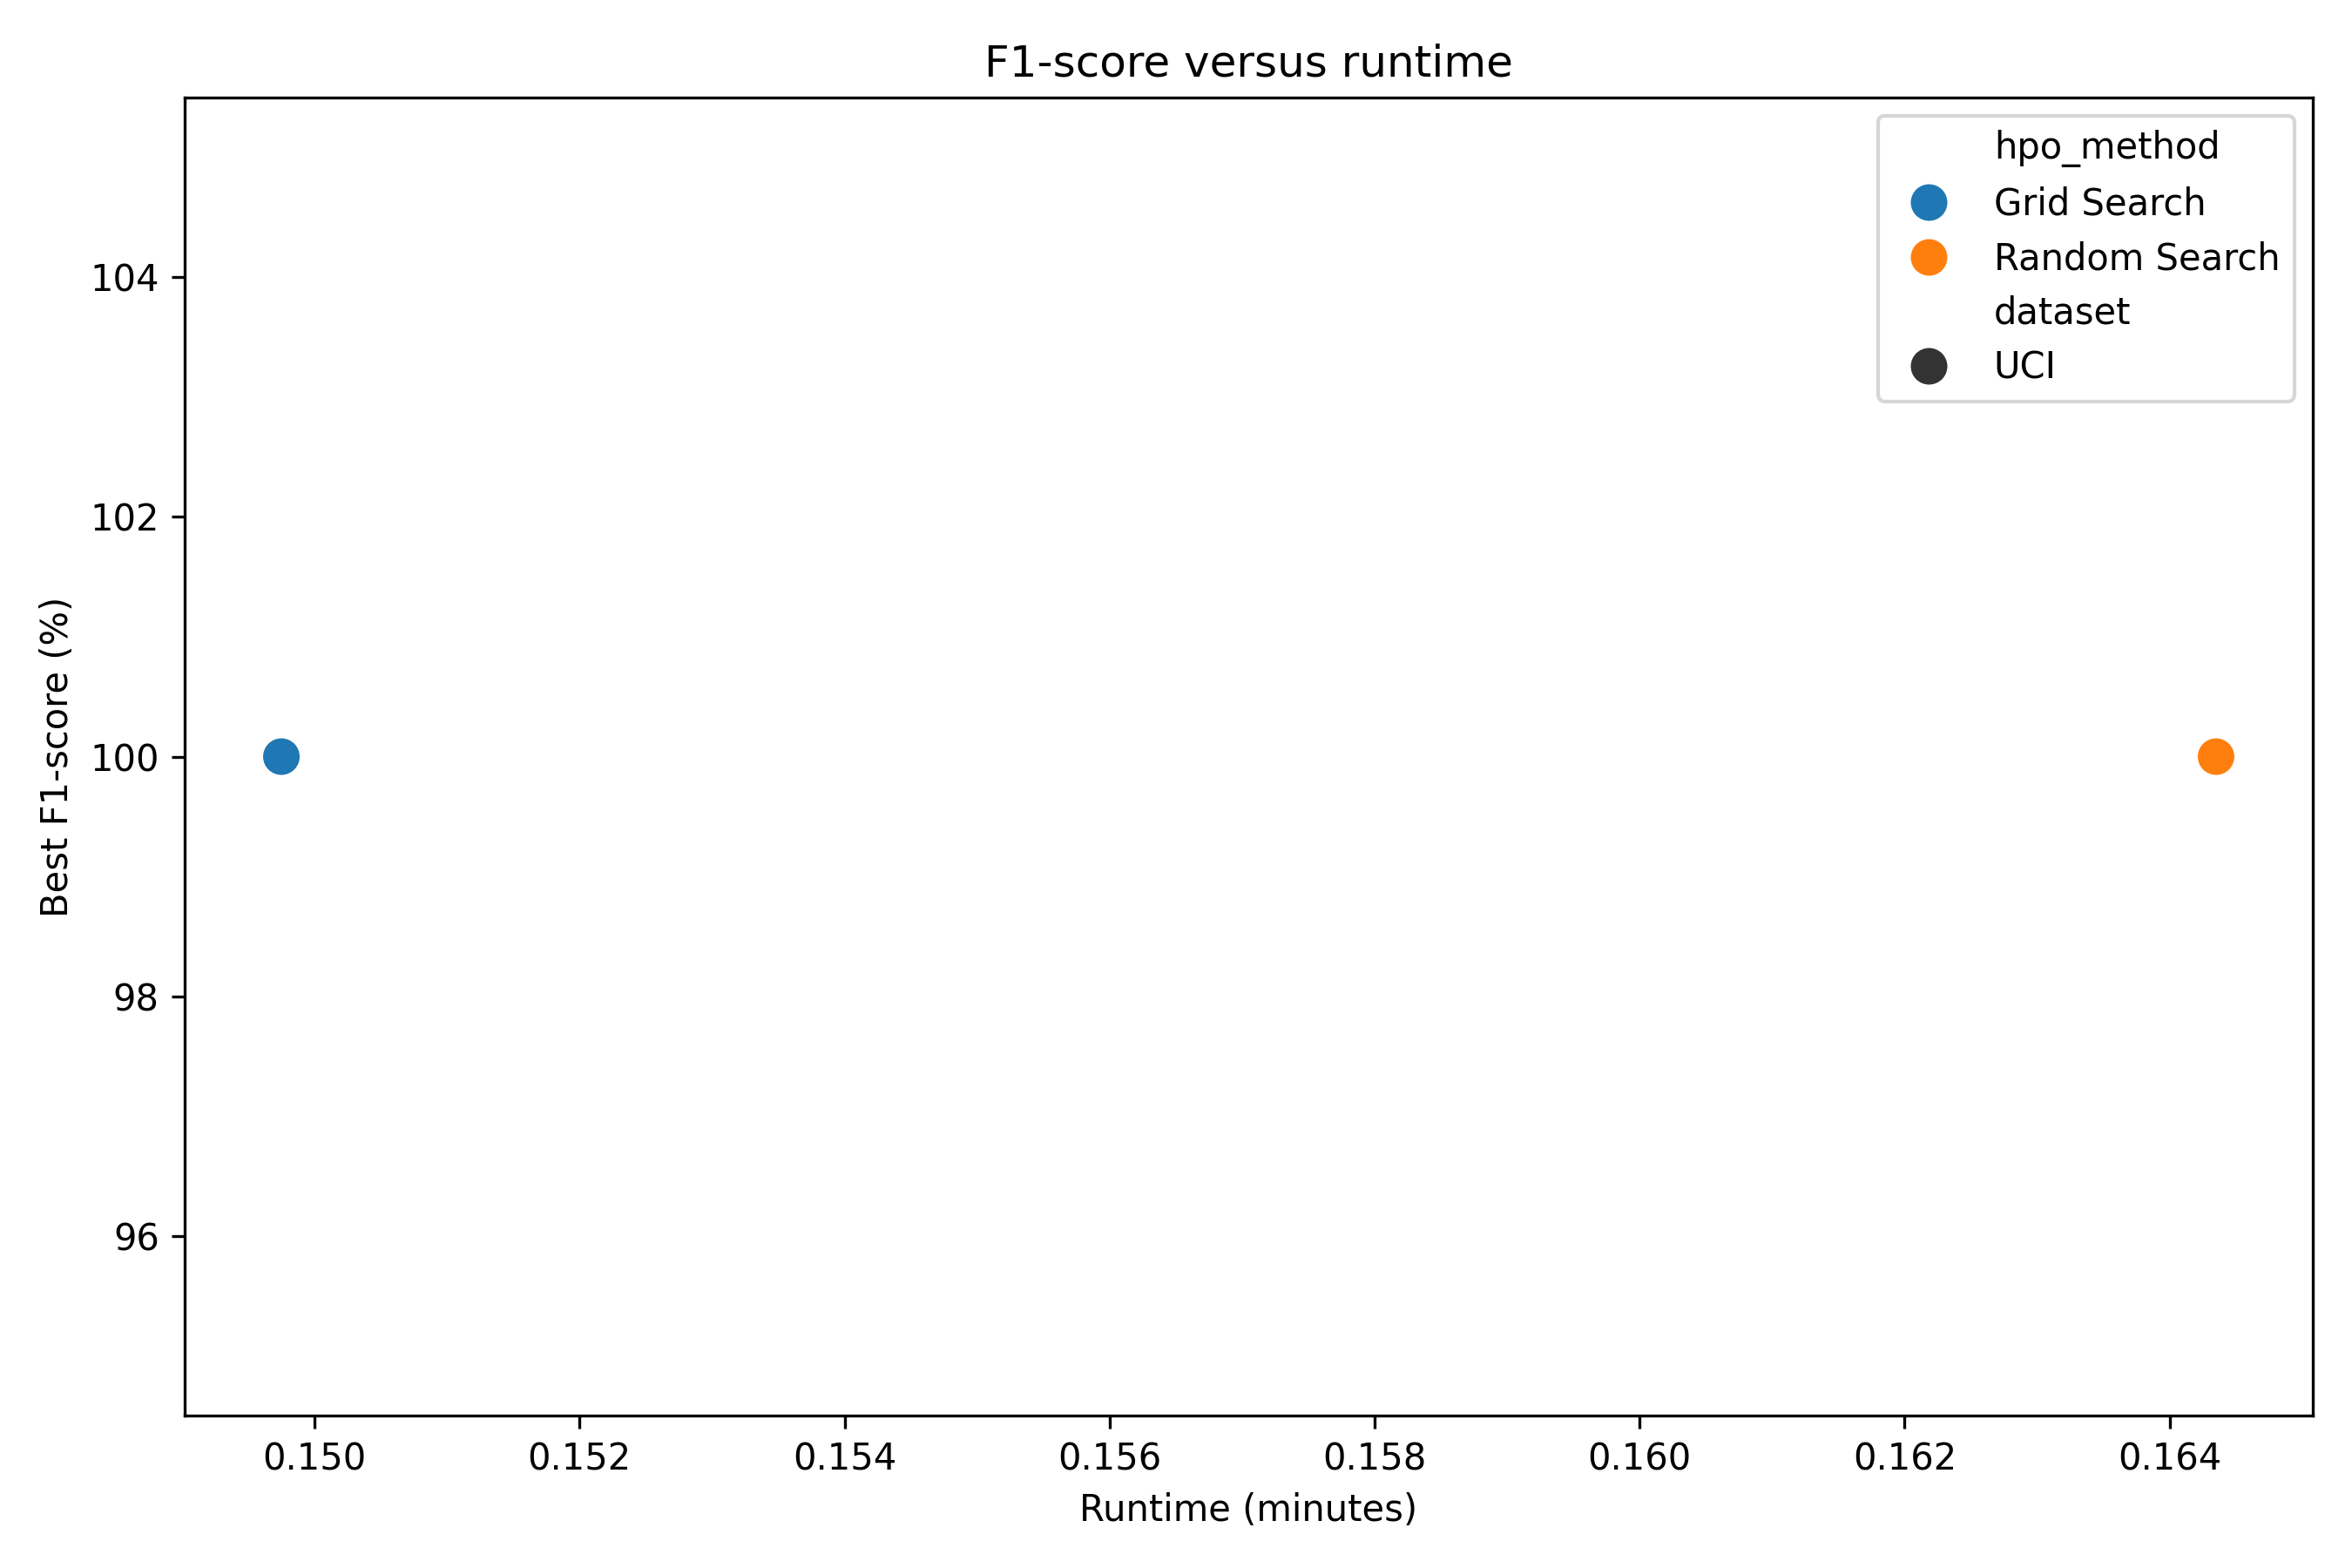
\includegraphics[width=0.85\linewidth]{figures/f1_vs_runtime.png}
\caption{Best verified UCI F1-score versus runtime for Grid Search and Random Search.}
\label{fig:f1_runtime}
\end{figure}

\begin{figure}[t]
\centering
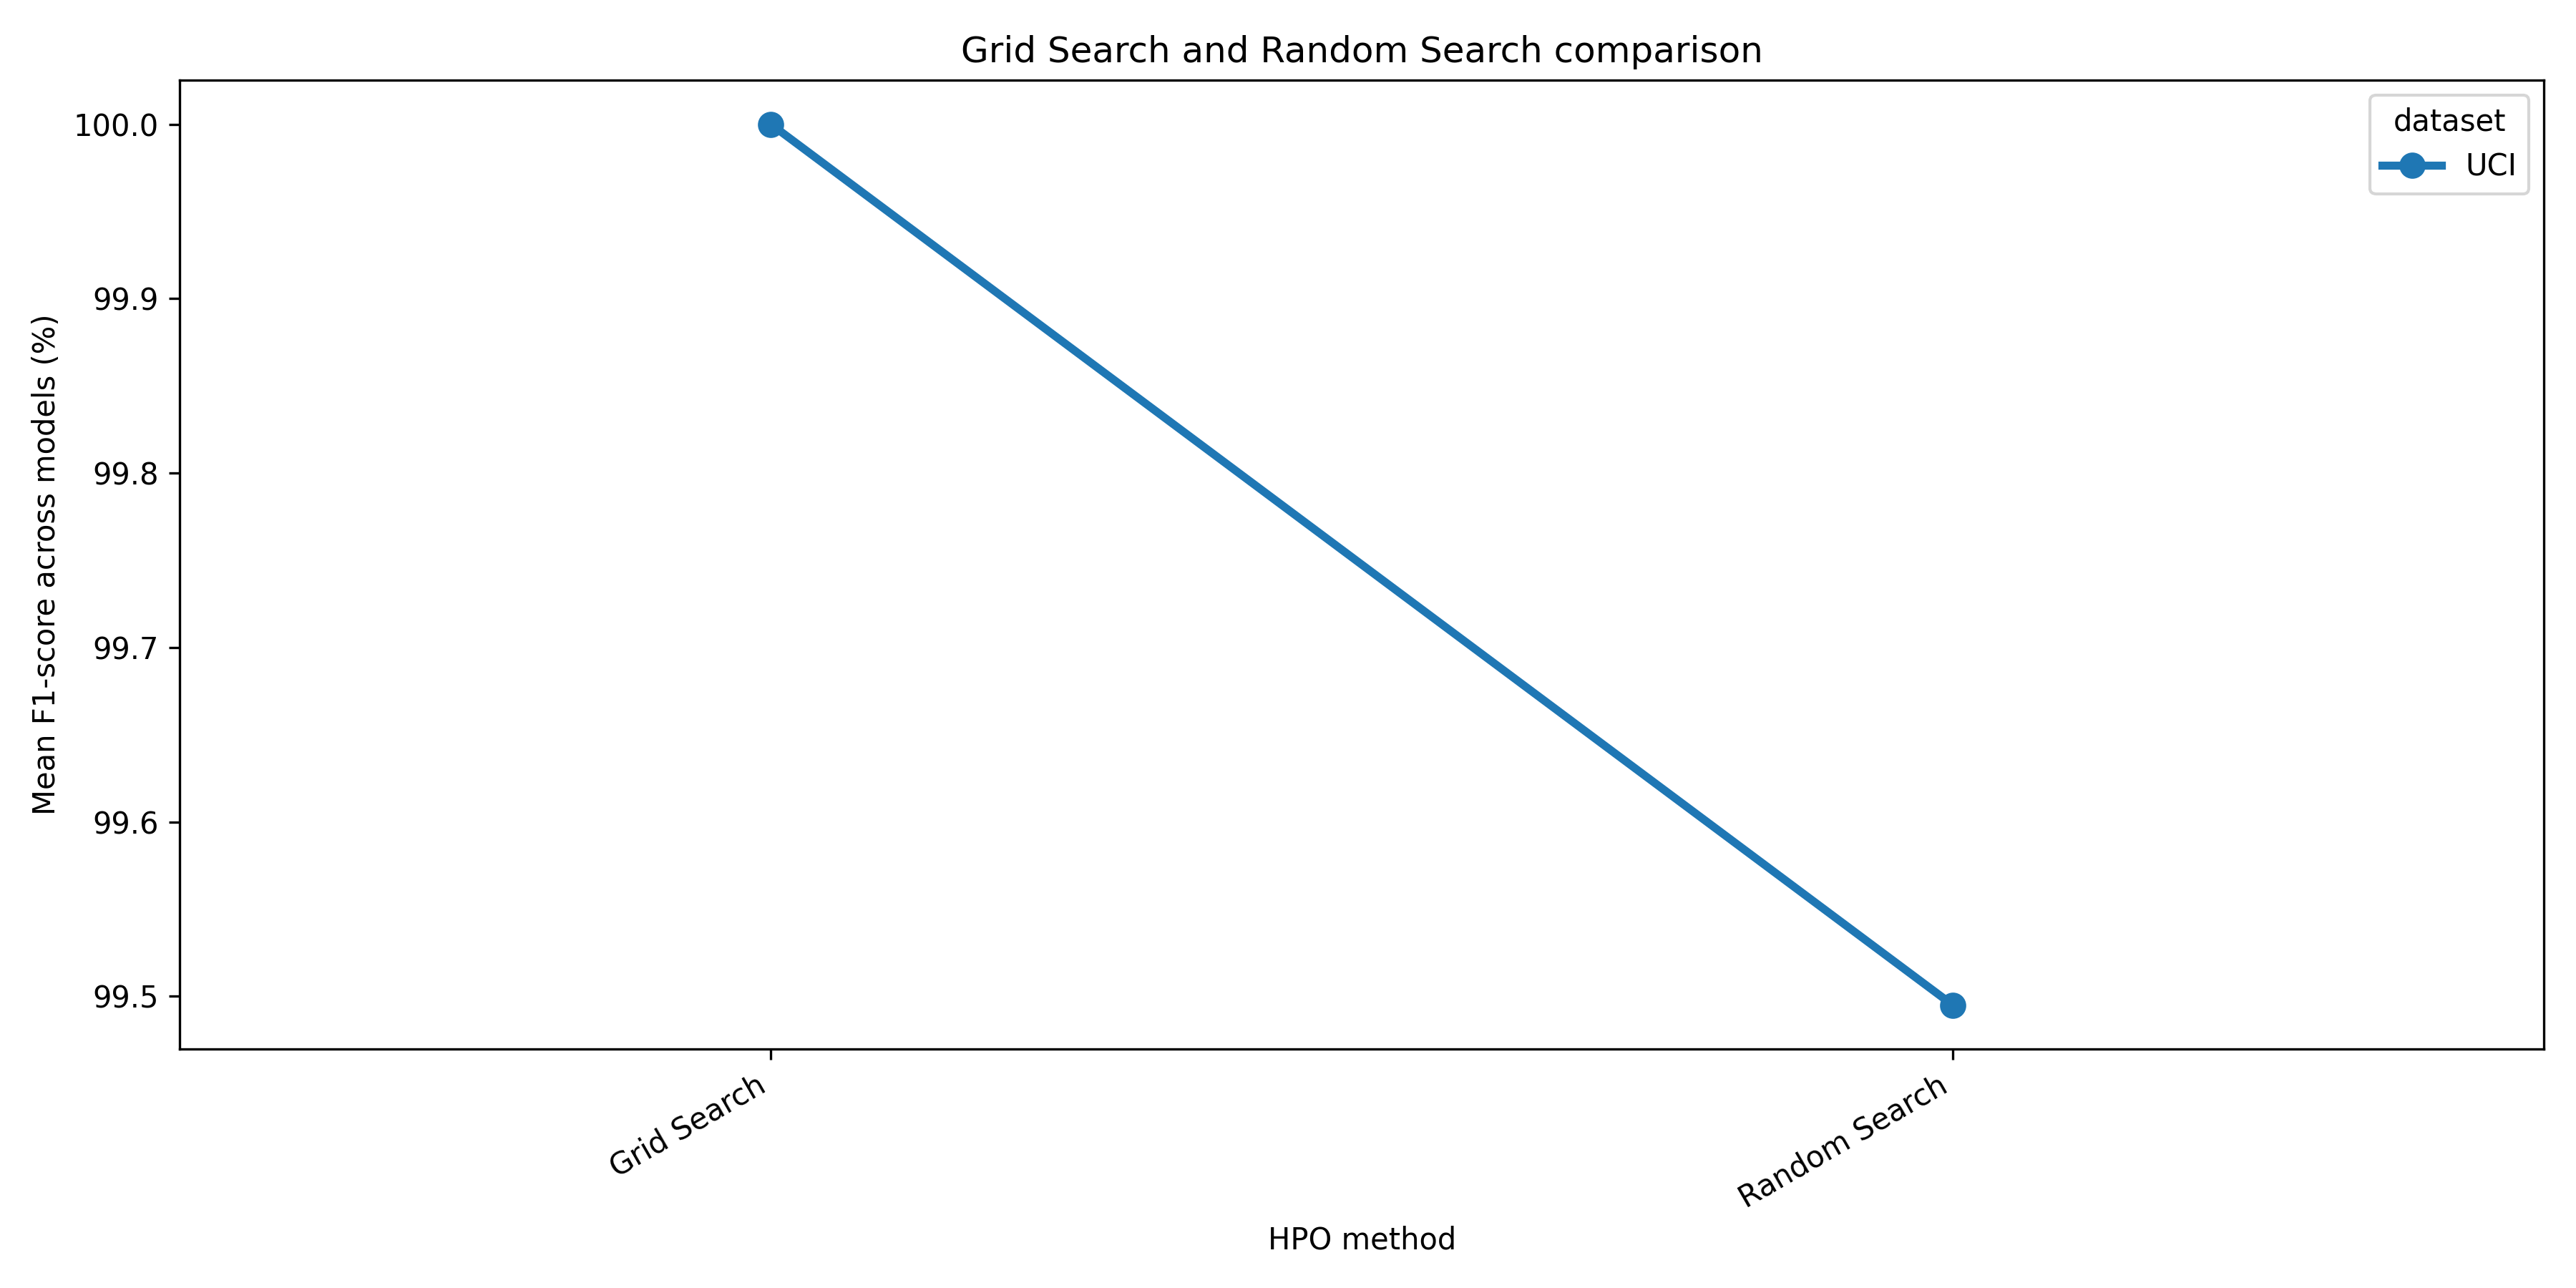
\includegraphics[width=0.95\linewidth]{figures/hpo_method_comparison.png}
\caption{Mean F1-score comparison of Grid Search and Random Search in the verified public UCI pipeline.}
\label{fig:hpo_comparison}
\end{figure}

\section{Statistical Validation}

For the UCI dataset, model performance was summarized using mean and standard deviation across stratified validation folds. This provides a limited estimate of variability under the selected validation design. For larger clinical data, additional repeated validation, temporal validation, site-level validation, and external validation would be required before making stronger generalization claims. Statistical comparisons should account for repeated measurements across folds and shared data splits.

\section{Limitations}

This study has several limitations. The UCI CKD dataset is small and may not represent the diversity of real clinical populations. The eICU cohort depends on local cohort construction choices and may not directly generalize to non-critical-care settings. The repository does not include raw clinical data because of licensing, privacy, and credentialing requirements. The current results summarize experimental model development and should not be interpreted as clinical validation.

For the eICU-derived analysis, CKD severity staging depends on the phenotype definition used to construct the cohort. CKD chronicity cannot be assumed from single ICU measurements because acute kidney injury, transient laboratory changes, and incomplete pre-admission history may affect renal markers. External clinical validation is therefore required before any clinical-use interpretation.

\section{Ethical Considerations}

CKD prediction models may influence clinical interpretation if used improperly. Any clinical use would require institutional review, privacy-preserving data handling, fairness assessment, external validation, calibration analysis, and clinician oversight. This repository is intended for research and reproducibility only. It does not provide a diagnostic tool or medical advice.

The study is intended to use only de-identified public or credentialed datasets, including public UCI data and credentialed eICU access through PhysioNet. The models are not intended for real-time clinical decision-making and should be viewed as research and decision-support experiments rather than autonomous diagnostic systems.

\section{Reproducibility Statement}

The experiments use random seed 42, 5-fold stratified cross-validation, equalized search budgets across HPO methods where applicable, and training-fold-only preprocessing. Results are reported as mean $\pm$ standard deviation when repeated validation estimates are available. Raw UCI and eICU datasets must be obtained from their official sources, and private clinical data must not be committed to the repository.

\section{Conclusion}

This study compared HPO methods for CKD prediction across a small public benchmark and a larger credentialed critical-care setting. In the verified public UCI pipeline, SVM achieved 100.0\% held-out F1-score under both Grid Search and Random Search, while Random Forest with Random Search reached 98.99\%. Random Search remained a practical method because it provided competitive performance with a compact search budget. The results emphasize that HPO strategy and runtime should be reported transparently in clinical machine learning studies.

\section{Future Scope}

Future work should include external validation across independent clinical sites, calibration assessment, decision-curve analysis, fairness evaluation, and explainability methods such as SHAP. Additional work should also examine temporal cohort definitions, missingness mechanisms, and robustness under different preprocessing strategies.

\nocite{*}
\bibliographystyle{splncs04}
\bibliography{references}

\end{document}
